\documentclass{article}
\usepackage{enumerate}
\usepackage{enumitem}
\usepackage{amsmath}
\usepackage{amssymb}
\usepackage{graphicx}


\begin{document}
\title{CSC361: Written Assignment 1 (w1)}
\author{Paul MacKay}

\maketitle

\section{}
\begin{enumerate}[label=(\alph*)]
%(for the lecture on access technologies) Internet access over telephone lines has been driven by your desire
%for higher speed. Given the following fact: voice bandwidth: 3,000 Hz; signal-to-noise ratio between two phone
%sets: 30 dB; modem sampling rate: 2,400 baud, please explain concisely:
%(a) how your old modem was improved from 2.4 to 9.6 and 28.8 Kbps (i.e., kilobit-per-second) in speed; [0.5]
	\item 
        We can explain how to increase the data rate from 2.4 to 9.6 and 28.8 Kbps using the concept of 
        bits-per-symbol. Using 1, 4, 12 bits/symbol respectively. Adding more bits/symbol increases 
        the data rate up to a certain point.
        Using the formula: 
        \begin{align*}
            data rate &= (bits/symbol) \times baud rate  \\
            data rate &= 1 \times 2400 = 2.4 Kbps  \\
            data rate &= 4 \times 2400 = 9.6 Kbps \\
            data rate &= 12 \times 2400 = 28.8 Kbps 
        \end{align*}

%(b) why such improvement stopped around 33.6 Kbps; [0.5]
	\item 
        According to the Shannon-Hartley theorem there exists a maximum data rate 
        which depends on noise level, bandwidth, and overall infrastructure. 
        Given these parameters the theorem states that 33.6 is the maximum limit 
        using the bits/symbol model.

%(c) how 56 Kbps is achieved otherwise; [0.5]
	\item 
        Due to the asymmetric demand for download/upload speeds i.e users download
        more data than they upload. The downstream can use more of the total bandwidth
        since the upstream uses less bandwidth. This utilization of bandwidth 
        for downstream allows for speeds up to 56 Kbps.

%(d) how your DSL modem or optical network terminal (ONT) now can achieve an even higher speed. [0.5]
	\item 
        ONTs solve many of the short comings by using light to transmit data rather than electrical signals.
        Some of the benefits of this technology is:
        \begin{itemize}
            \item ONTs are capable of carrying much more bandwidth than traditional wires.
            \item Reduced noise.
            \item Symmetrical downstream/upstream.
        \end{itemize}
\end{enumerate}
%
%2. (for the lectures on HTTP) A simplified HTML document is at http://a.b.com/index.html
%<html><a href=”fig/tiny.gif’’><img src=’’fig/small.gif’’></a>
%<img src=’’http://x.y.com/fig/big.gif’’>
%<img src=’’http://a.b.com/fig/huge.gif’’></html>
%Please show your work. For a web browser that loads images (GIF files) automatically, how long (in round-trip
%time) does it take, excluding the DNS overhead, to display the entire Web page if all files are small enough to
%be accommodated in one packet and:
%(a) non-persistent, non-parallel HTTP connections are used [0.5], or
%(b) non-persistent HTTP connections with at most two parallel connections are used [0.5], or
%(c) persistent, non-parallel HTTP connections without pipelining are used [0.5], or
%(d) persistent, non-parallel HTTP connections with pipelining are used. [0.5]
\newpage
\section{}
\emph{see work on next page}
\begin{enumerate}[label=(\alph*)]
    \item 8 RTTs
    \item 4 RTTs
    \item 4 RTTs
    \item 2 RTTs
\end{enumerate}
\section{}

\subsection{Pros}
\begin{itemize}
    \item Faster speeds in rural areas when compared with existing technology. 
    \item Provides internet without the need of huge cable infrastructure. (good for connecting 
        third world countries)
\end{itemize}

\subsection{Cons}
\begin{itemize}
    \item Less delay than GEO satellites but is highly variable, 20 - 80 ms.
    \item In some regions longer and more staged delay 100 - 400 ms
\end{itemize}

\begin{figure}[h]
  \centering
  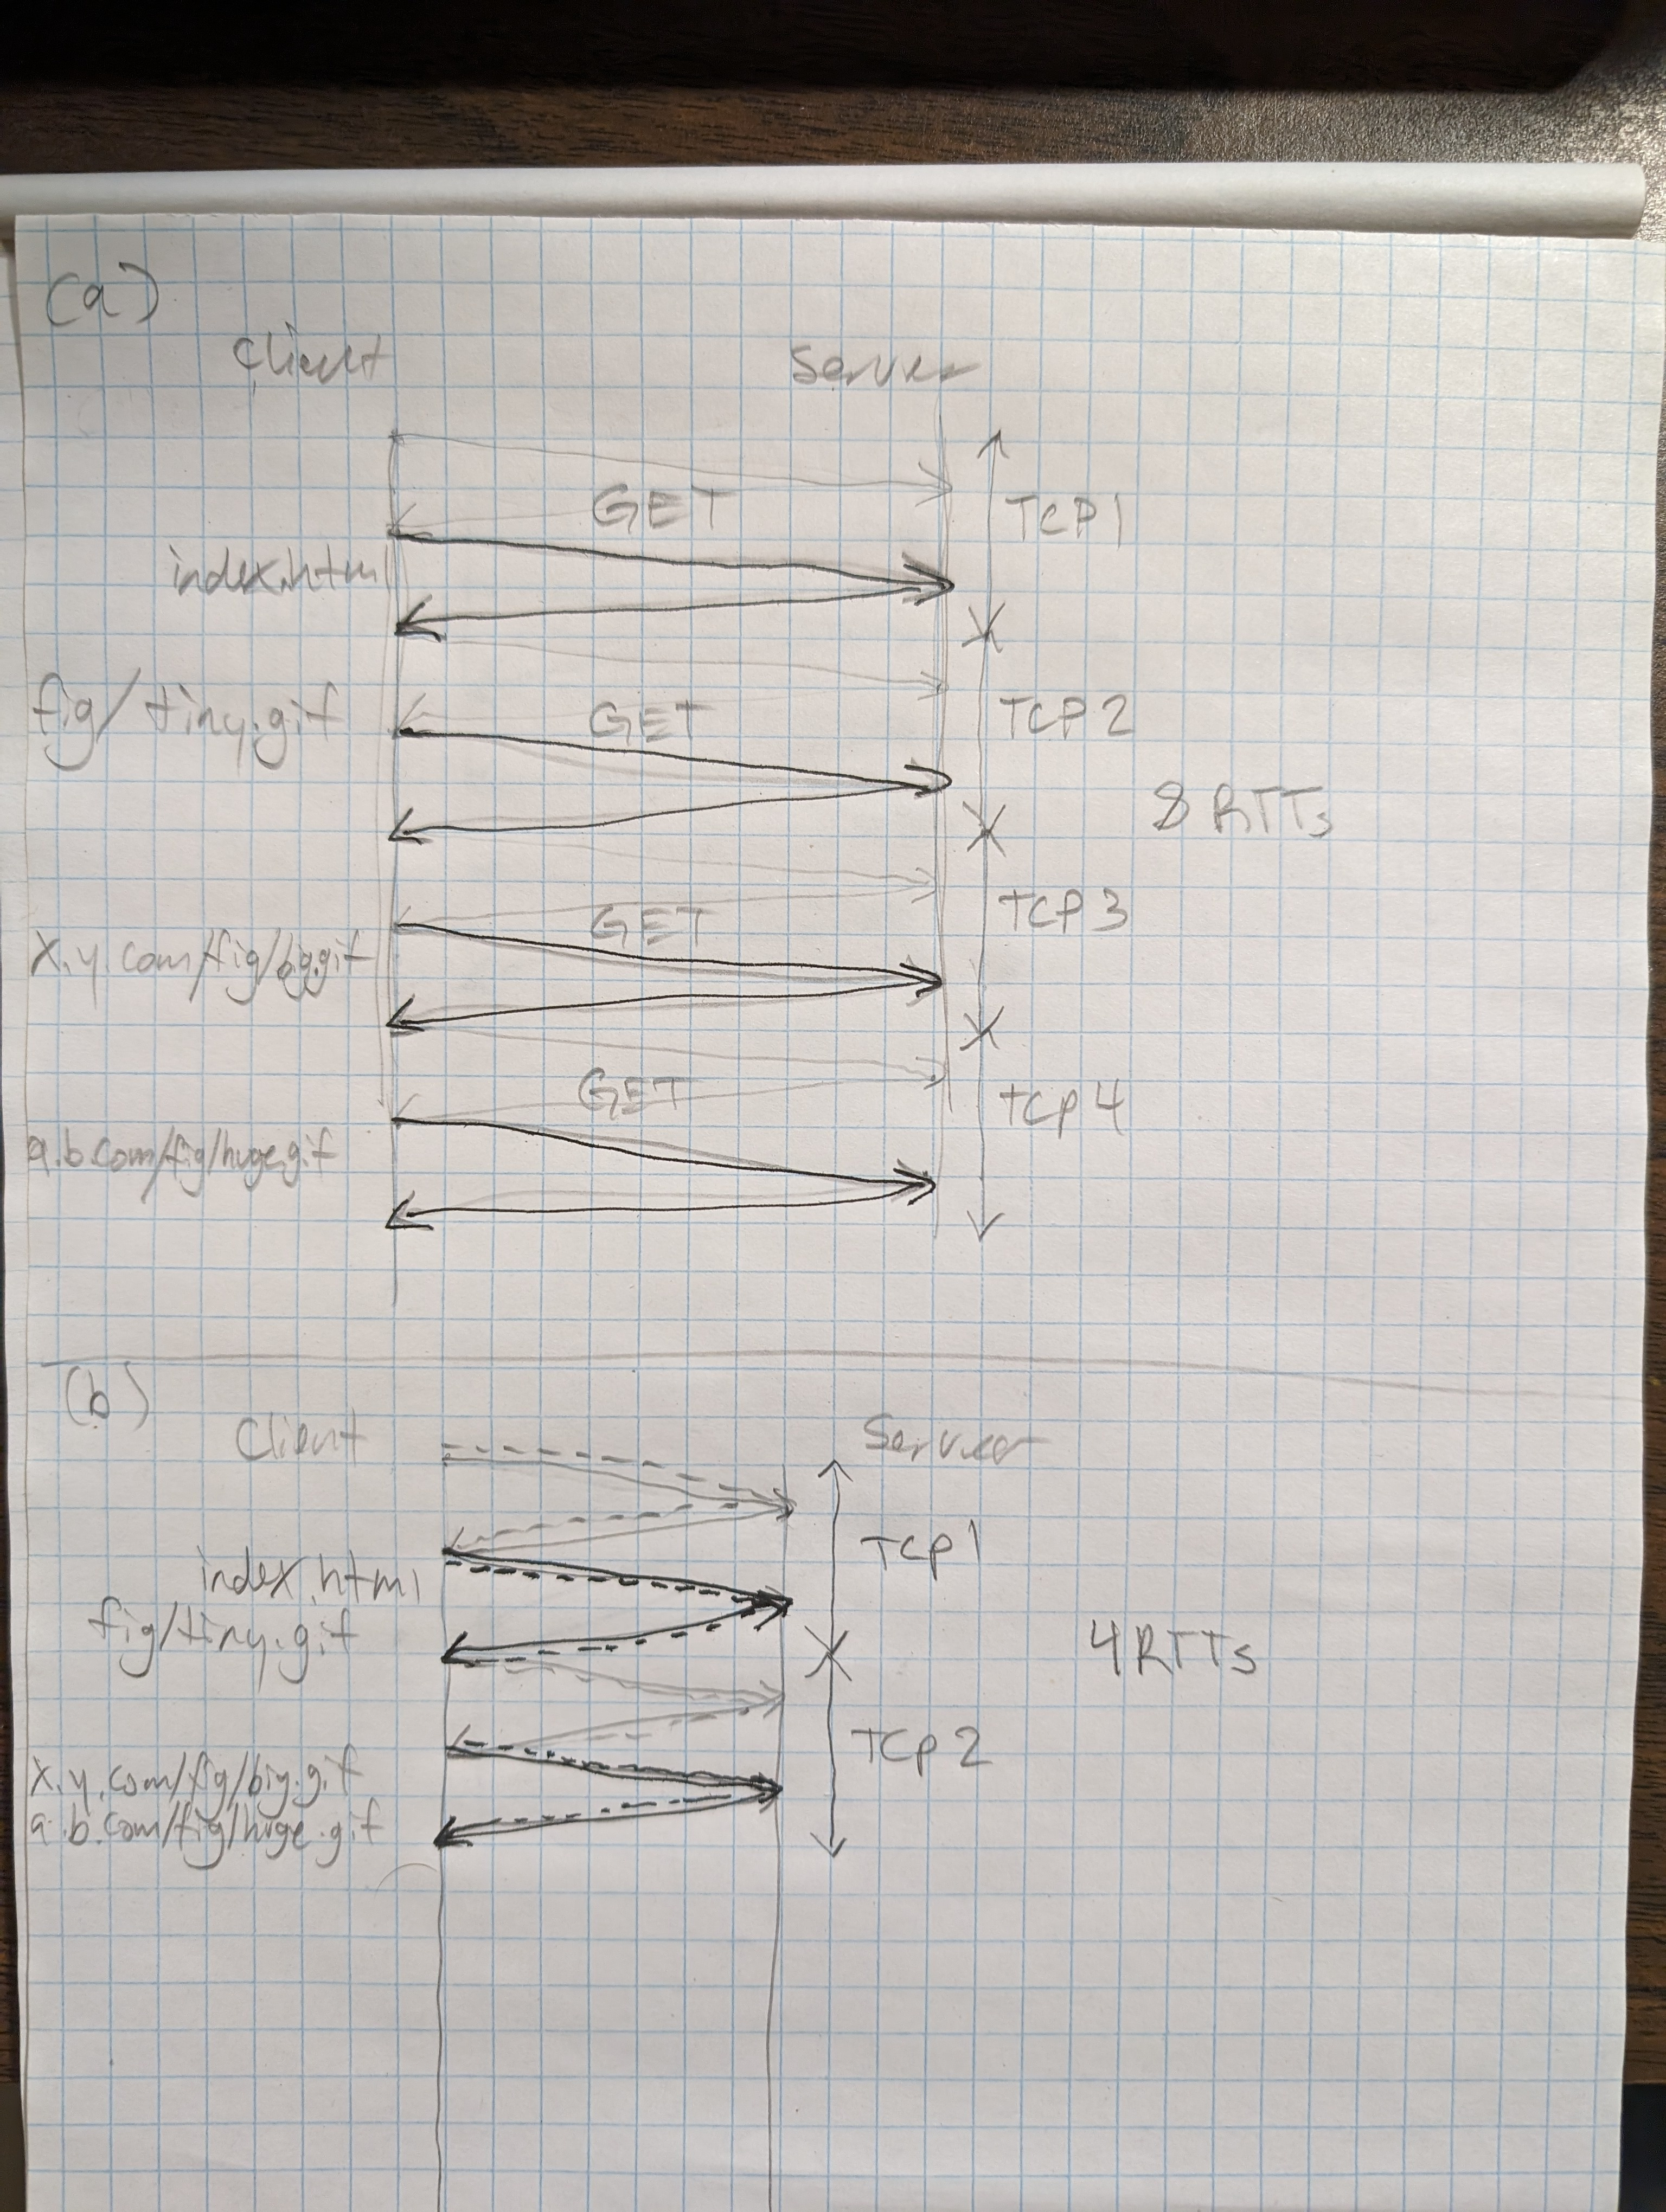
\includegraphics[width=\textwidth]{1.jpg}
\end{figure}

\begin{figure}[h]
  \centering
  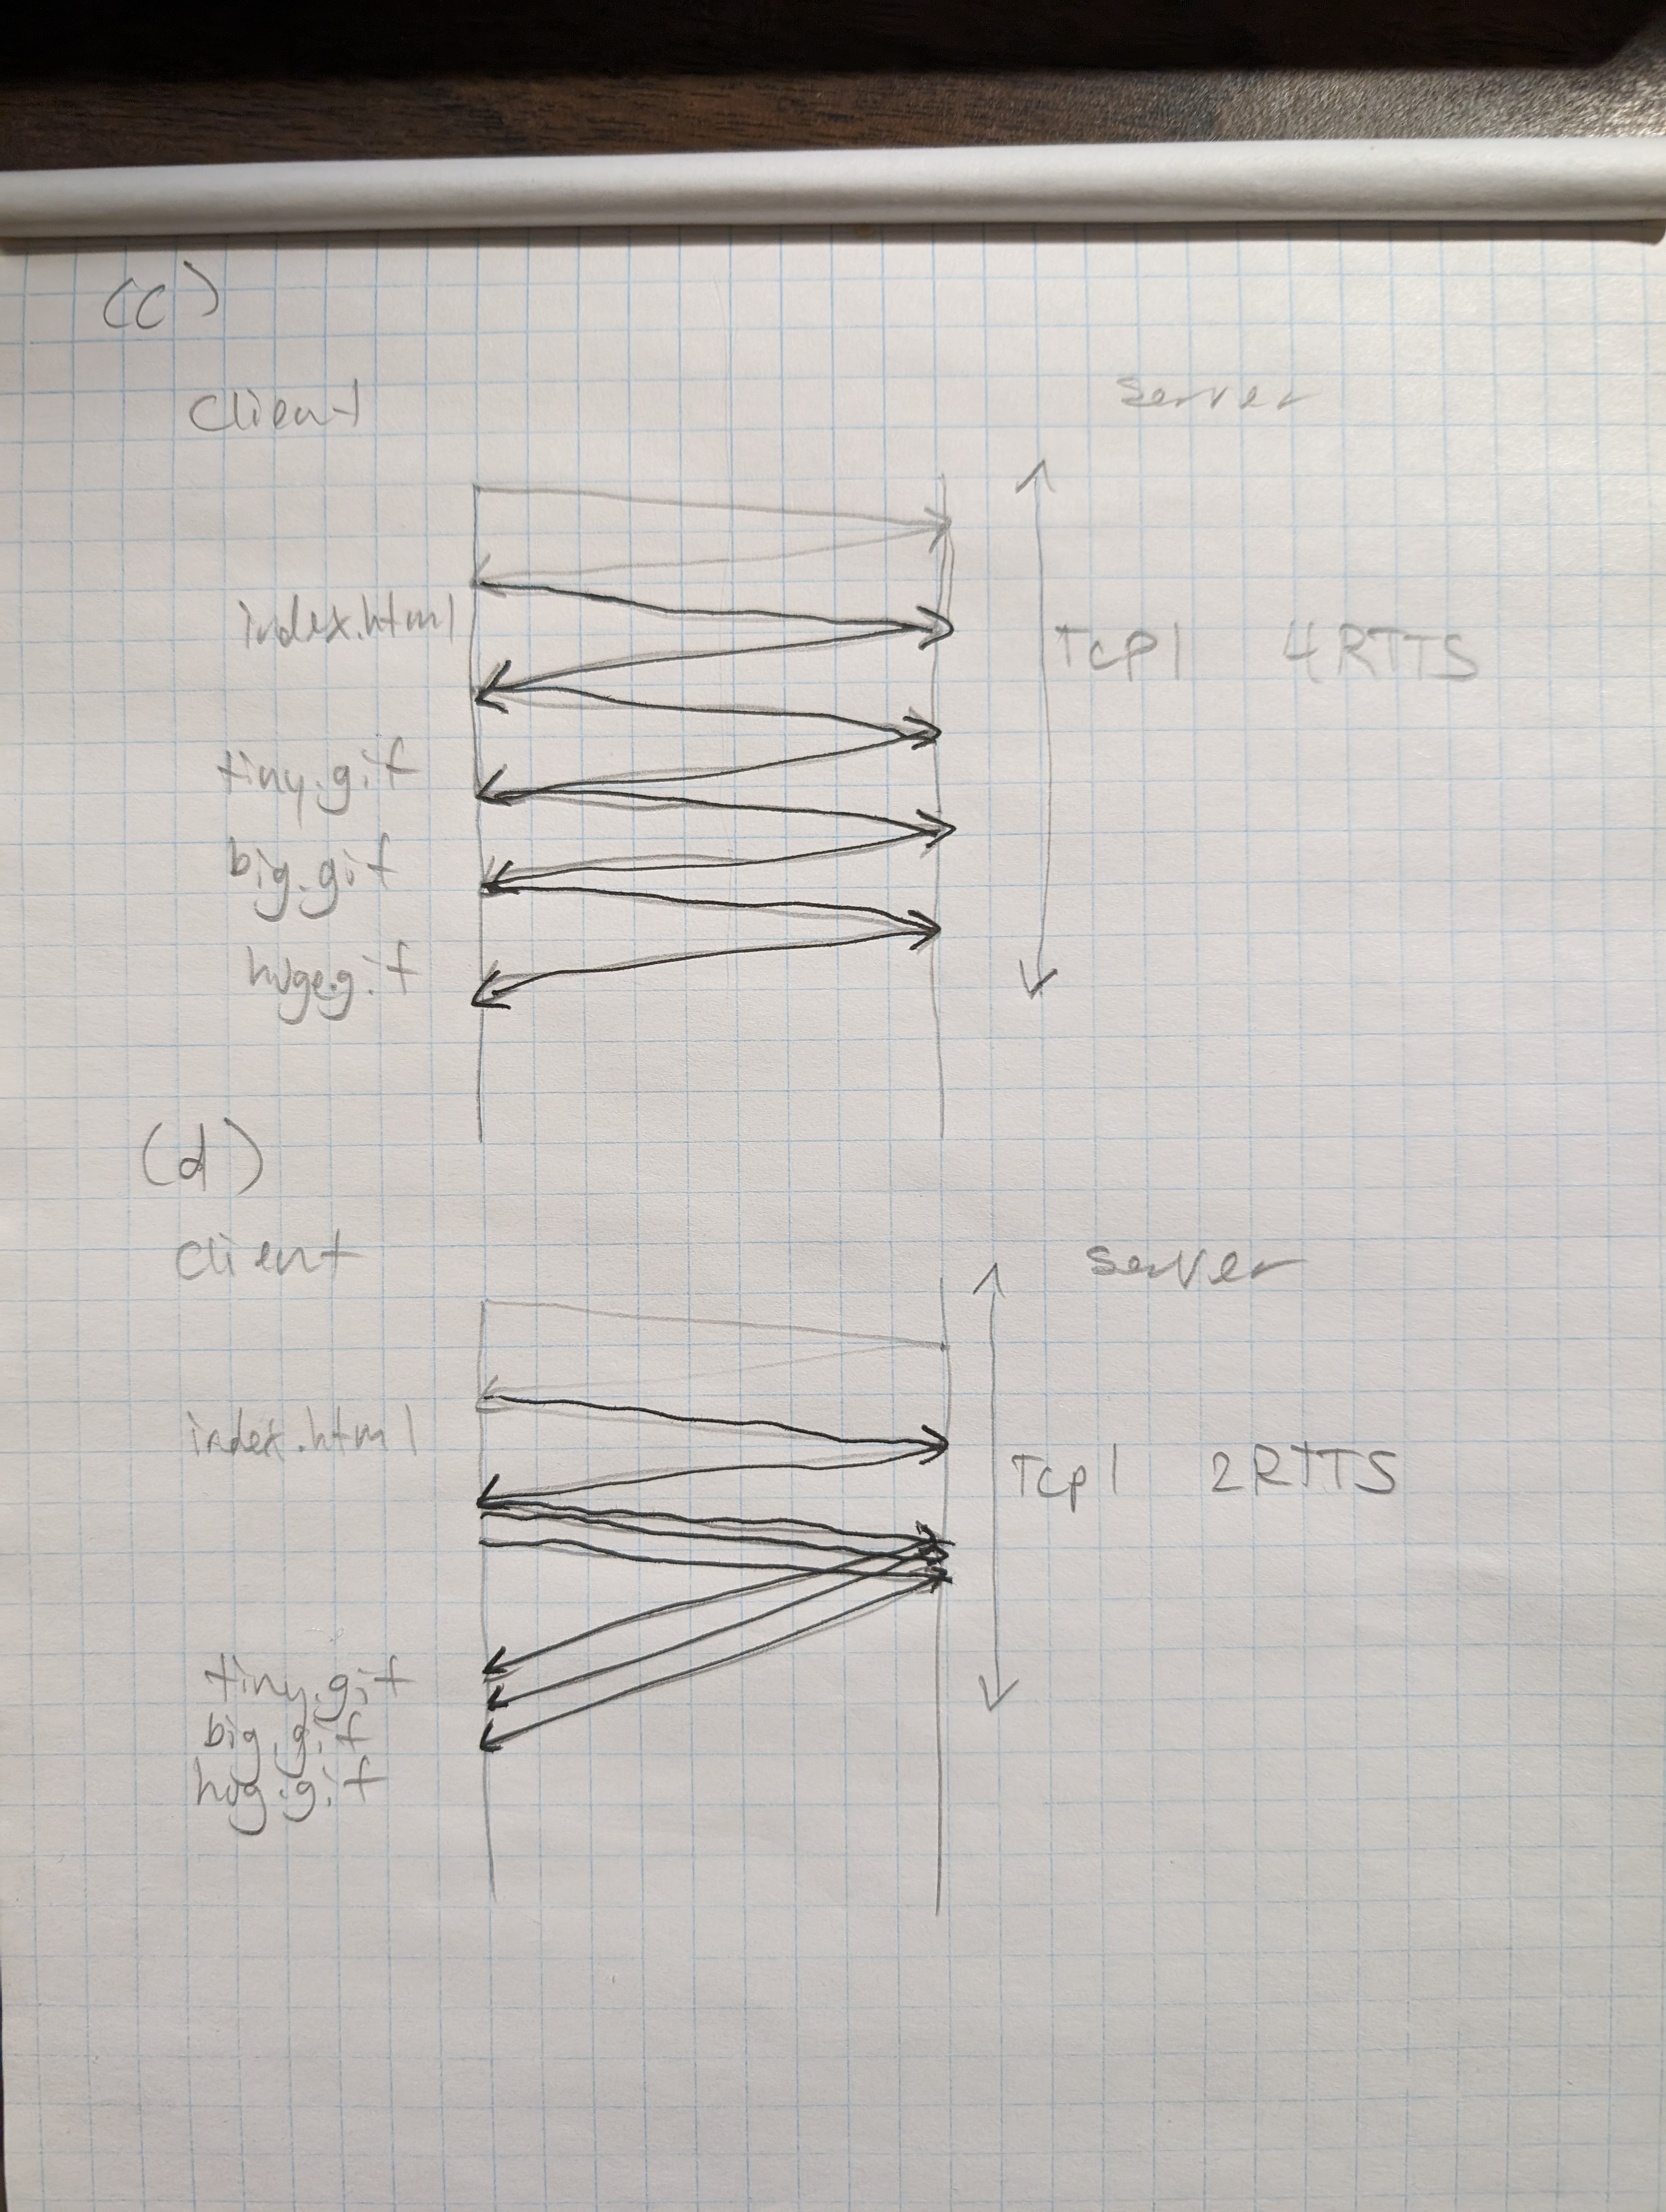
\includegraphics[width=\textwidth]{2.jpg}
\end{figure}



\end{document}
